\chapter{Calculating areas in the simplex}\label{appen:AreaSimplex}
In Chapter~\ref{chp:1}, we characterize the behavior of the competitive community by considering the area encircled by the system’s trajectory on the simplex. Because of the noisy character of the dynamics in the stochastic simulations, the amplitude of the oscillations is not a robust indicator. Instead, if the system fluctuates with small amplitude around some equilibrium abundances, the trajectory occupies a small area (Figure~\ref{chp1:fig:3}c), whereas larger oscillations would cover broader areas (Figure~\ref{chp1:fig:3}a,b). Here we add details on how we compute the area encircled by the trajectory.\\

We have run $50$ realizations of our $3$-species system for every radius. For each simulation, the trajectory can be interpreted as points in a 3D space (gray dots in Figure~\ref{fig:areaExplained}, where the averaged density triplet $(\overline{x}_1,\overline{x}_2,\overline{x}_3)$  is the middle cross). To characterize the trajectory, we aim to measure the area covered by those points. \\

For programming convenience, it is more practical to change to a two-dimensional space $(y_1,y_2)$. The chosen space is the one defined by the $x +y +z = 1$  plane, as the density triplets always lie on it because $\sum_{i}^{g} x_i(t) = 1$ at all times. Let $(\hat{u},\hat{v})$ be two vectors in that plane that form an orthonormal basis. In particular:
\begin{equation}
    \hat{u} = \sqrt{\frac{1}{2}} \begin{pmatrix}
           -1 \\
           1 \\
           0
         \end{pmatrix} , \;
    \hat{v} = \sqrt{\frac{2}{3}} \begin{pmatrix}
           -1/2 \\
           -1/2 \\
           1
         \end{pmatrix}.
\end{equation}
The areas in each space are conserved because the transformation is isometric. In turn, the change of coordinates of our points is given by:
\begin{equation}
    y_1 = (x_1,x_2,x_3)\sqrt{\frac{1}{2}} \begin{pmatrix}
           -1 \\
           1 \\
           0
         \end{pmatrix} , \;
     y_2 = (x_1,x_2,x_3)\sqrt{\frac{2}{3}} \begin{pmatrix}
           -1/2 \\
           -1/2 \\
           1
         \end{pmatrix}.
\end{equation}
During the simulation, heavy fluctuations may occur, but the densities there do not represent the typical behavior of the ecosystem. These extreme densities are the outermost points of the set of points that populate the two-dimensional space. To get a representative area, we eliminate those boundary points, more precisely, we remove the $5\%$ of outlier points. We then calculate the area enclosed by the polygon defined by the new outermost points (green line in Figure~\ref{fig:areaExplained}) using \texttt{MATLAB}'s function  \texttt{polyarea} \cite{polyarea}.

\begin{figure}
    \centering
    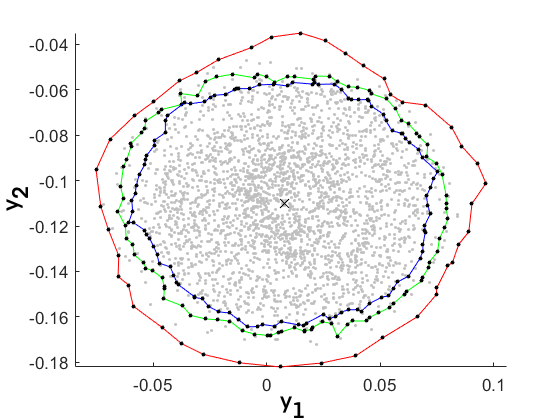
\includegraphics[width=\textwidth]{figures/appendices/area_explainedy.png}
    \caption[Calculating areas in the simplex]{Trajectory points in the $2$D of a simulation of a RGG with $10^4$ nodes and $R_{RGG} = 0.03$. The red line encloses all the points. Green and blue lines enclose the $95\%$ and $90\%$ of the points, respectively.}
    \label{fig:areaExplained}
\end{figure}

